%% Præsentation for C-programmering for begyndere
%% Lavet af Jacob Bechmann Pedersen og Jacob Skjødt Nielsen
%% For C undervisning i IDA 
%%
%% Theme: `DarkConsole'
%% Copyright (c) 2011-2017 Kazuki Maeda <kmaeda@kmaeda.net>
%% Distributable under the MIT License:
%% http://www.opensource.org/licenses/mit-license.php 

%% Preamble
\documentclass{beamer}

\usepackage{hyperref} % Add a link to your document
\usepackage{graphicx} % Add pictures to your document
\usepackage{listings} % Source code formatting and highlighting
\usepackage[utf8]{inputenc} % Gives UTF-8 encoded characters such as Æ, Ø, Å.

%% Setting the C language type, for viewing pleasure:
\usepackage{listings}
\usepackage{color}

\definecolor{link}{HTML}{CF55E3}
\definecolor{dkgreen}{rgb}{0,0.6,0}
\definecolor{gray}{rgb}{0.5,0.5,0.5}
\definecolor{arduinoBlue}{HTML}{33CCCC}
\definecolor{arduinoOrange}{HTML}{FF9900}
\definecolor{arduinoGray}{HTML}{669999}

\lstset{frame=tb,
  inputencoding=utf8,
  language=C,
  aboveskip=3mm,
  belowskip=3mm,
  showstringspaces=false,
  columns=flexible,
  basicstyle={\small\ttfamily},
  numbers=left,
  numbersep=0pt,
  keywordsprefix={\#, \<},
  numberstyle=\tiny\color{gray},
  keywordstyle=\color{C_darkblue},
  commentstyle=\color{dkgreen},
  stringstyle=\color{C_lightblue},
  breaklines=true,
  breakatwhitespace=true,
  tabsize=3,
  extendedchars=true,
  literate={æ}{{\ae}}1 {ø}{{\o}}1 {å}{{\r a}}1 {Æ}{{\AE}}1 {Ø}{{\O}}1 {Å}{{\r A}}1,
}

\usetheme{C_Console}
\title{C-Programmering for begyndere}
\date{23. april 2018}
\subtitle{Del 4 - Microcontrollerprogrammering, Arduino, Hardware og physical computing}
\author{Jacob B. Pedersen\footnote{jacob.bp@mvb.net} og Jakob S. Nielsen\footnote{jakob990@gmail.com}}

%% Document
\begin{document}

\begin{frame}
	\maketitle
\end{frame}

\begin{frame}{Indhold}
	\tableofcontents
\end{frame}

\section{Repetition}
\subsection{Hvad lavede vi sidste gang?}

%%----------------------------------------------------------------------
\begin{frame}[fragile]{Hvad lavede vi sidste gang? - Libraries}
	\begin{itemize}
		\item{Vi skrev vores egne funktioner}
		\item{Satte dem i libraries}
		\begin{itemize}
			\item{Lærte at bruge headers og implementationsfiler:}
			\begin{itemize}
				\item{{\color{dkgreen}.h} og {\color{dkgreen}.c}}
			\end{itemize}
		\end{itemize}
			\begin{center}
				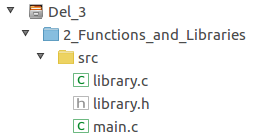
\includegraphics[height=0.2\textheight]{assets/libraries.png}
			\end{center}
			\begin{lstlisting}
				#include "library.h"
			\end{lstlisting}
			\begin{lstlisting}
				#ifndef LIBRARY_H
				#define LIBRARY_H

				// Prototype af multiply funktionen:
				int multiply(int x, int y);

				#endif /* LIBRARY_H */
			\end{lstlisting}
	\end{itemize}
\end{frame}
%%----------------------------------------------------------------------

%%----------------------------------------------------------------------
\begin{frame}[fragile]{Hvad lavede vi sidste gang? - Arrays}
	\begin{itemize}
		\item{Vi blev klogere på {\color{dkgreen}arrays}}
		\begin{itemize}
			\item{Og hvordan vi holdt tekststrenge i {\color{C_darkblue}char arrays}}
			\item{Arrays kunne også holde lister af {\color{C_darkblue}int} eller {\color{C_darkblue}float}}
		\end{itemize}
		\begin{center}
				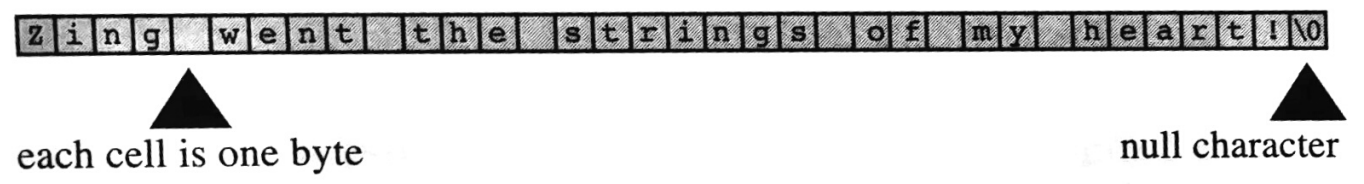
\includegraphics[width=0.7\textwidth]{assets/char_array.png}
		\end{center}
		\begin{lstlisting}
		char string[numberOfChars]; // Char array
		int intArray[number of ints]; // Integer array 
		float floArray[number of floats]; // Float array 
		\end{lstlisting}
	\end{itemize}
\end{frame}
%%----------------------------------------------------------------------

%%----------------------------------------------------------------------
\begin{frame}[fragile]{Hvad lavede vi sidste gang?- Typedef, enum}
	\begin{itemize}
		\item{Vi fik også lært at repræsentere data vha. egne datatyper:}
		\begin{itemize}
			\item{{\color{C_darkblue}typedef} gav en datatype et alias}
			\item{{\color{C_darkblue}enum} gav integer værdier navne i stedet}
		\end{itemize}
		\begin{lstlisting}
		// Et smart eksempel på enums kunne være at gøre en fysisk udregning overskuelig:
		typedef float length;
		typedef float width;
		typedef float height;
		typedef float volume;

		// Enums kunne være gode til at skelne mellem ting som f.eks. farve:
		enum color { red, orange, yellow, green, blue, purple };
		\end{lstlisting}
	\end{itemize}
\end{frame}
%%----------------------------------------------------------------------

%%----------------------------------------------------------------------
\begin{frame}[fragile]{Hvad lavede vi sidste gang? - Structs, unions}
	\begin{itemize}
		\item{Til sidst organiserede vi data vha. {\color{C_darkblue}structs} og {\color{C_darkblue}unions}}
		\begin{itemize}
			\item{{\color{C_darkblue}structs} var en samling af data}
			\begin{lstlisting}
			struct book{
				char title[40]; // Bogens titel
				char author[40]; // Bogens forfatter
				float price; // Bogens pris
				int stars; // Bogens rating fra 1-5
				};
			\end{lstlisting}
			\item{{\color{C_darkblue}union} kunne antage mere end én type}
			\begin{lstlisting}
			union varchar{
				int digit;
				double bigFloat;
				char letter;
				};
			\end{lstlisting}
		\end{itemize}
	\end{itemize}
\end{frame}
%%----------------------------------------------------------------------

\section{I dag}
\subsection{Dagens program}

%%----------------------------------------------------------------------
\begin{frame}[fragile]{Dagens program}
\begin{itemize}
	\item{I dag skal vi se på programmering af microcontrollers!}
	\item{Arduino er den hurtigste af slagsen at gå til!}
	\item{Vi skal have installeret {\color{arduinoBlue}Arduino IDE}}
	\item{Lære om {\color{arduinoBlue}Arduino} funktioner:}
	\begin{itemize}
		\item{{\color{arduinoOrange}pinMode}(), {\color{arduinoOrange}delay}(), {\color{arduinoOrange}digitalRead}() mfl.}
	\end{itemize}
	\item{Hvordan vi bruger det sammen med vores nuværende C-viden og kobler det på omverdenen!}
\end{itemize}
\end{frame}
%%----------------------------------------------------------------------

\subsection{Hvad er Arduino}
%%----------------------------------------------------------------------
\begin{frame}[fragile]{Hvad er Arduino?}
\begin{columns}
\begin{column}{0.5\textwidth}
\begin{itemize}
	\item{{\color{arduinoBlue}Arduino} er et forsøg på at gøre microcontrollers lette at programmere i C.}
	\item{Microcontrollers er enheder, der indholder alle delene i en lille computer}
	\item{Bygget specielt til at styre anden elektronik vha. software}
	\item{Arduinoen giver dette inteface gennem sine "pins" som vist:}
\end{itemize}
\end{column}
\begin{column}{0.5\textwidth}
	\begin{center}
		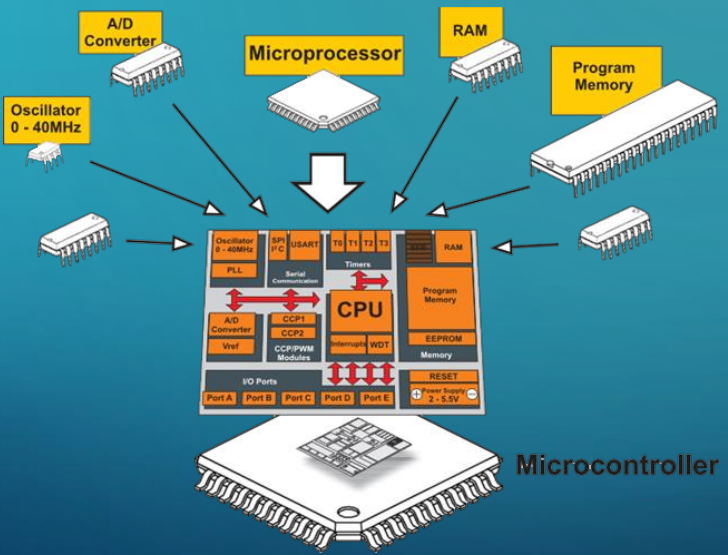
\includegraphics[width=0.5\textwidth]{assets/microcontroller.png}
	\end{center}
	\begin{center}
		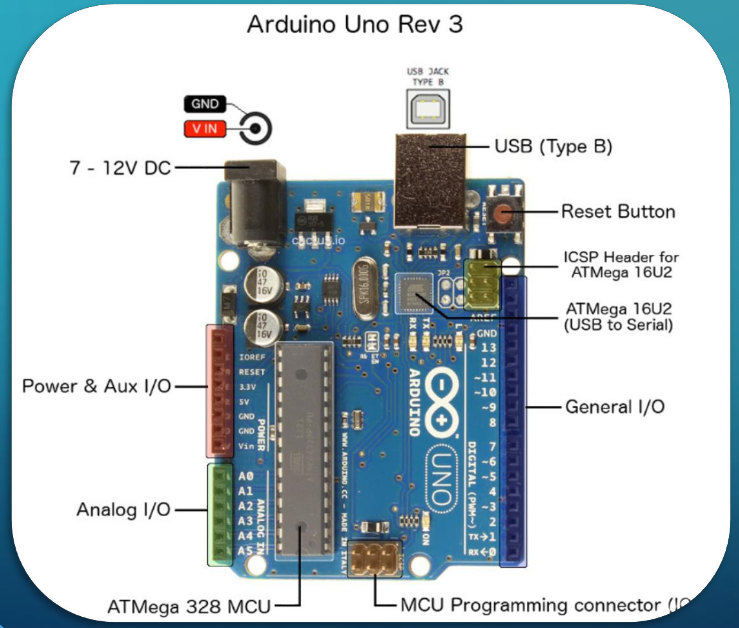
\includegraphics[width=0.9\textwidth]{assets/arduino_layout.png}
	\end{center}
\end{column}
\end{columns}
\end{frame}
%%----------------------------------------------------------------------

\subsection{Installation af Arduino IDE}

%%----------------------------------------------------------------------
\begin{frame}[fragile]{Installation af Arduino IDE}
\begin{itemize}
	\item{Gå ind på {\color{link}\href{https://arduino.cc/download/}{https://arduino.cc/download/}}
	\item{Vælg versionen til dit OS, og tryk "{\color{arduinoGray}Just download}", når de beder om donationer}
	\item{Kør installeren og sig ja til alle drivers!}
\end{itemize}
\end{frame}
%%----------------------------------------------------------------------

\subsection{Introduktion til Arduino-funktionerne}

%%----------------------------------------------------------------------
\begin{frame}[fragile]{Introduktion til Arduino-funktionerne}
	\begin{itemize}
		\item{Arduino IDE indeholder faktisk blot en skjult C compiler}
		\item{Den skriver C "lidt om" for at gøre Microcontrollere lettere for nybegyndere}
		\item{Det hele gøres vha. {\color{arduinoBlue}"arduino.h"} som er automatisk {\color{dkgreen}#include}'d}
		\item{en af de vigtigste forskelle er at den fjerner {\color{C_darkblue}main}(), og erstatter den med dette:}
		\begin{lstlisting}
			void setup(){
				// Kode der kører en gang i starten af Arduino programmet
			}
			void loop(){
				// Kode der kører i ring resten af tiden.
			}
		\end{lstlisting}
	\end{itemize}
\end{frame}
%%----------------------------------------------------------------------

%%----------------------------------------------------------------------
\begin{frame}[fragile]{Introduktion til Arduino-funktionerne}
	\begin{itemize}
		\item{Det betyder i virkeligheden bare:}
		\begin{lstlisting}
			int main(void){
				// Koder der kører i starten af programmet
				
				while(1){
					// Kode der kører i ring resten af tiden.
				}
				return 0;
			}
		\end{lstlisting}
	\end{itemize}
\end{frame}
%%----------------------------------------------------------------------

%%----------------------------------------------------------------------
\begin{frame}[fragile]{Introduktion til Arduino-funktionerne}
	\begin{itemize}
		\item{Arduino behandler typisk to former af fysisk data:}
		\item{Digital:}
		\begin{center}
		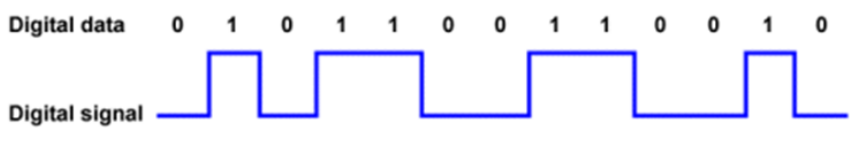
\includegraphics[height=0.1\textheight]{assets/digital_data.png}
	\end{center}
		\item{Analog:}
		\begin{center}
		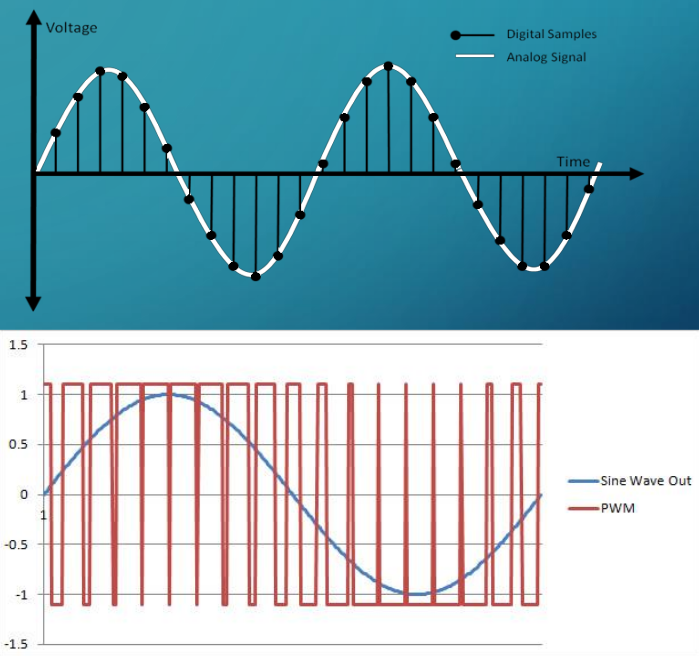
\includegraphics[height=0.7\textheight]{assets/analog_data.png}
	\end{center}
	\end{itemize}
\end{frame}
%%----------------------------------------------------------------------

%%----------------------------------------------------------------------
\begin{frame}[fragile]{Introduktion til Arduino-funktionerne}
	\begin{itemize}
		\item{En kort oversigt over nogle af Arduinos vigtigste funktioner:}
		\begin{lstlisting}
		pinMode(pin, mode); // Mode kan være enten INPUT, eller OUTPUT i det fleste tilfælde, 	men også INPUT_PULLUP, som er god til trykknapper.
		digitalRead(pin); // Læser digital værdi – true eller false, 1, 0, HIGH, LOW, fra pin.
		digitalWrite(pin, value); //  Value kan gives som true, false, 1, 0, eller HIGH og LOW.
		analogRead(analogPin); // Læser en værdi fra 0-1023 fra en analog pin A0-6
		analogWrite(pwmPin, value); // Skriver et PWM signal til en PWM pin (semi analogt signal)
		delay(milliseconds); // Bremser processoren i en tidsperiode, for at vente med næste handling.
		\end{lstlisting}
	\end{itemize}
\end{frame}
%%----------------------------------------------------------------------

\subsection{Blinky}

%%----------------------------------------------------------------------
\begin{frame}[fragile]{Blinky}
\begin{columns}
	\begin{column}{0.5\textwidth}
	\begin{itemize}
		\item{Blinky er Arduinos "Hello World"}
		\item{Vi skal kun bruge Arduinoen selv}
		\item{Og et kabel til at uploade sketchen!}
	\end{itemize}
	\end{column}
	\begin{column}{0.5\textwidth}
	\begin{center}
		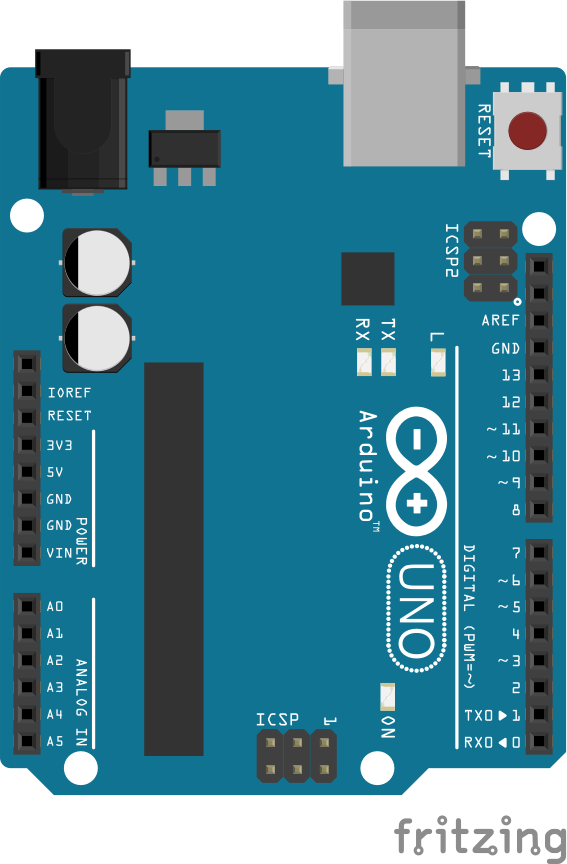
\includegraphics[width=0.7\textwidth]{../Examples/1_Blinky/1_Blinky_bb.png}
	\end{center}
	\end{column}
\end{columns}
\end{frame}
%%----------------------------------------------------------------------

\subsection{Input/Output}

%%----------------------------------------------------------------------
\begin{frame}[fragile]{Input/Output}
\begin{columns}
	\begin{column}{0.5\textwidth}
	\begin{itemize}
		\item{Nu kobler vi selv en LED på}
		\item{Vi tilføjer også en trykknap med pulldown}
		\begin{itemize}
			\item{Betyder at den som udgangspunkt læses som false/LOW}
		\end{itemize}
	\end{itemize}
	\end{column}
	\begin{column}{0.5\textwidth}
	\begin{center}
		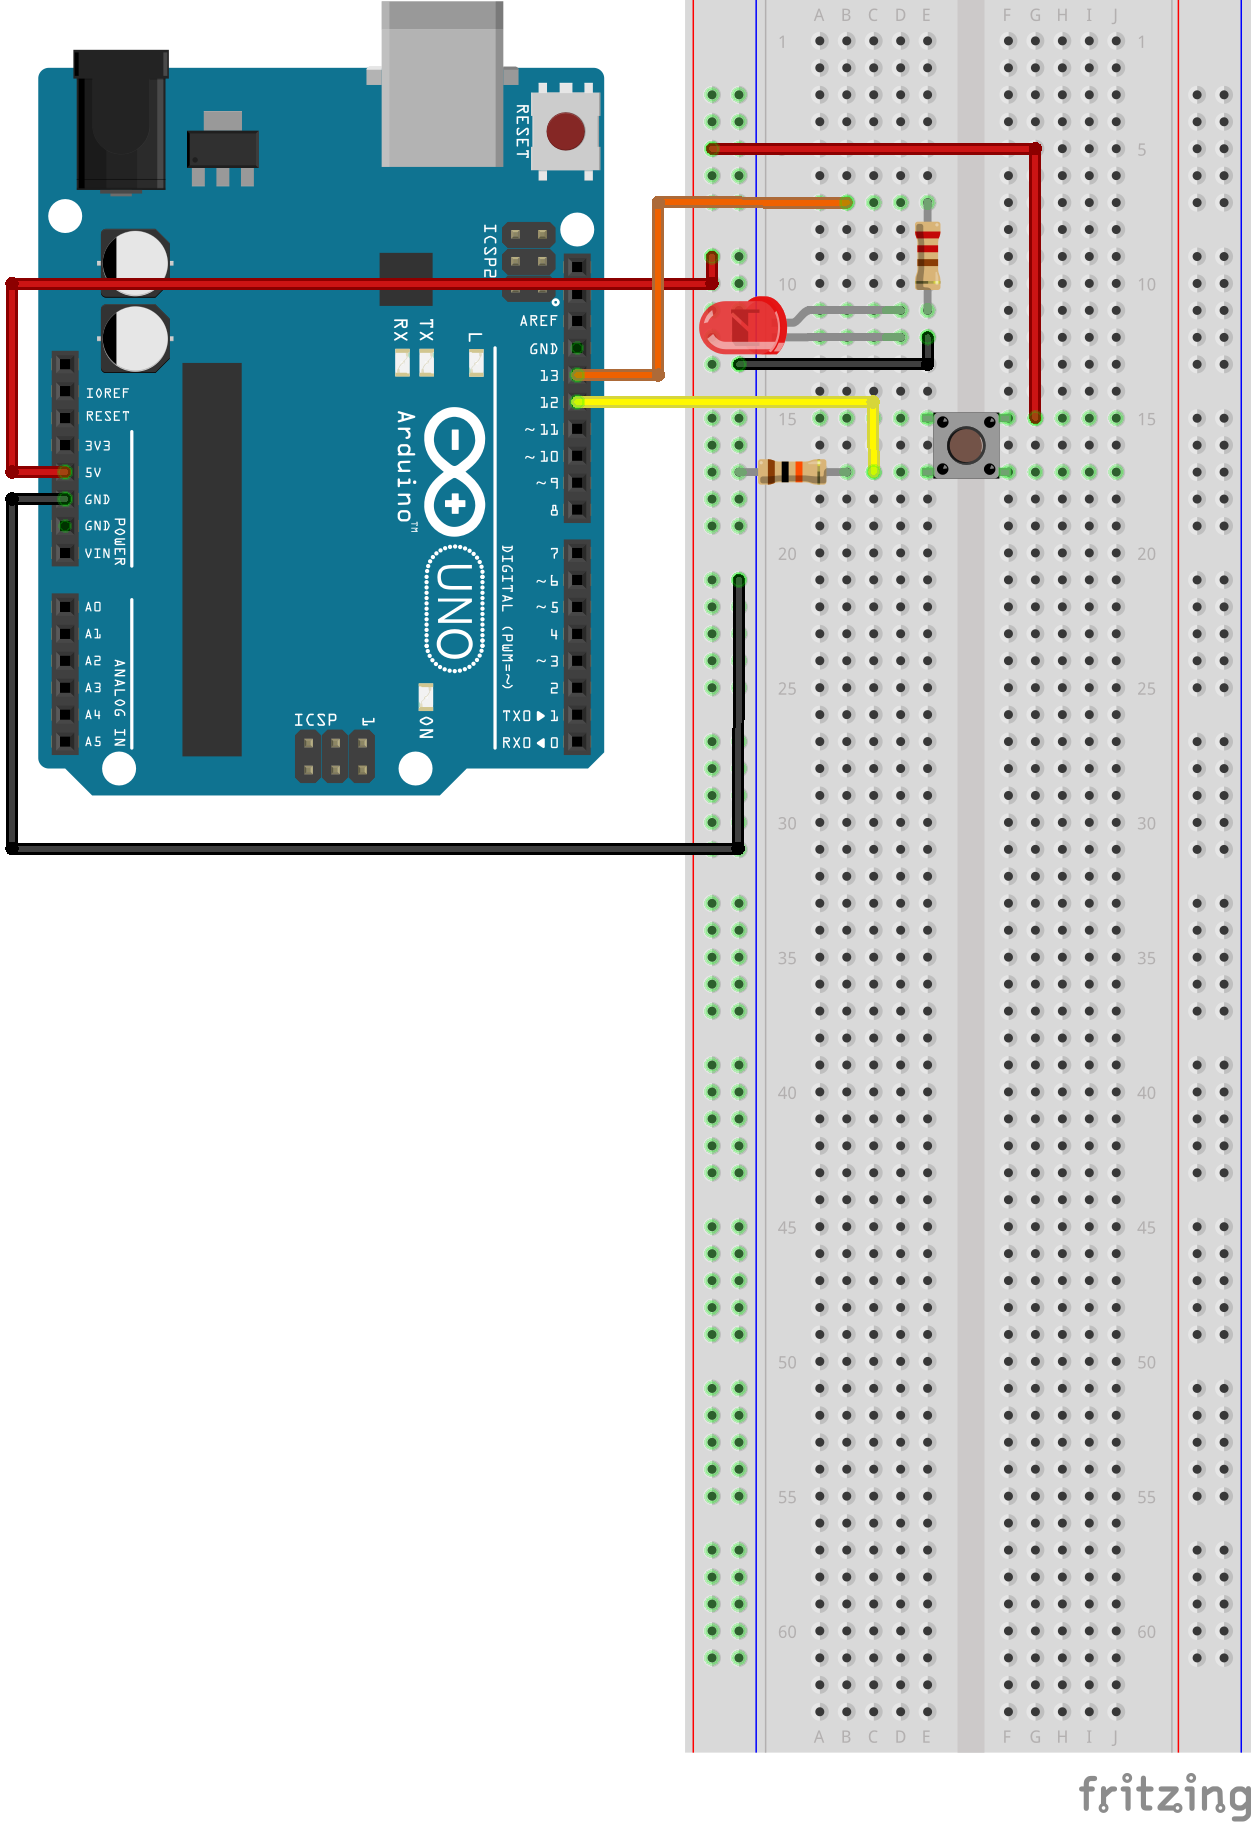
\includegraphics[width=1\textwidth]{../Examples/2_IO/2_IO_bb.png}
	\end{center}
	\end{column}
\end{columns}
\end{frame}
%%----------------------------------------------------------------------

\subsection{Analog I/O}

%%----------------------------------------------------------------------
\begin{frame}[fragile]{Input/Output}
\begin{columns}
	\begin{column}{0.5\textwidth}
	\begin{itemize}
		\item{Vi kigger også lidt på den analoge måde at gøre det}
		\item{I stedet for en trykknap bruger vi nu et potentiometer}
		\begin{itemize}
			\item{Den kan ændre den analoge spænding henover sig fra 0-5V}
		\end{itemize}
		\item{Vi styre LED'ens spænding med den og en PWM udgang!}
	\end{itemize}
	\end{column}
	\begin{column}{0.5\textwidth}
	\begin{center}
		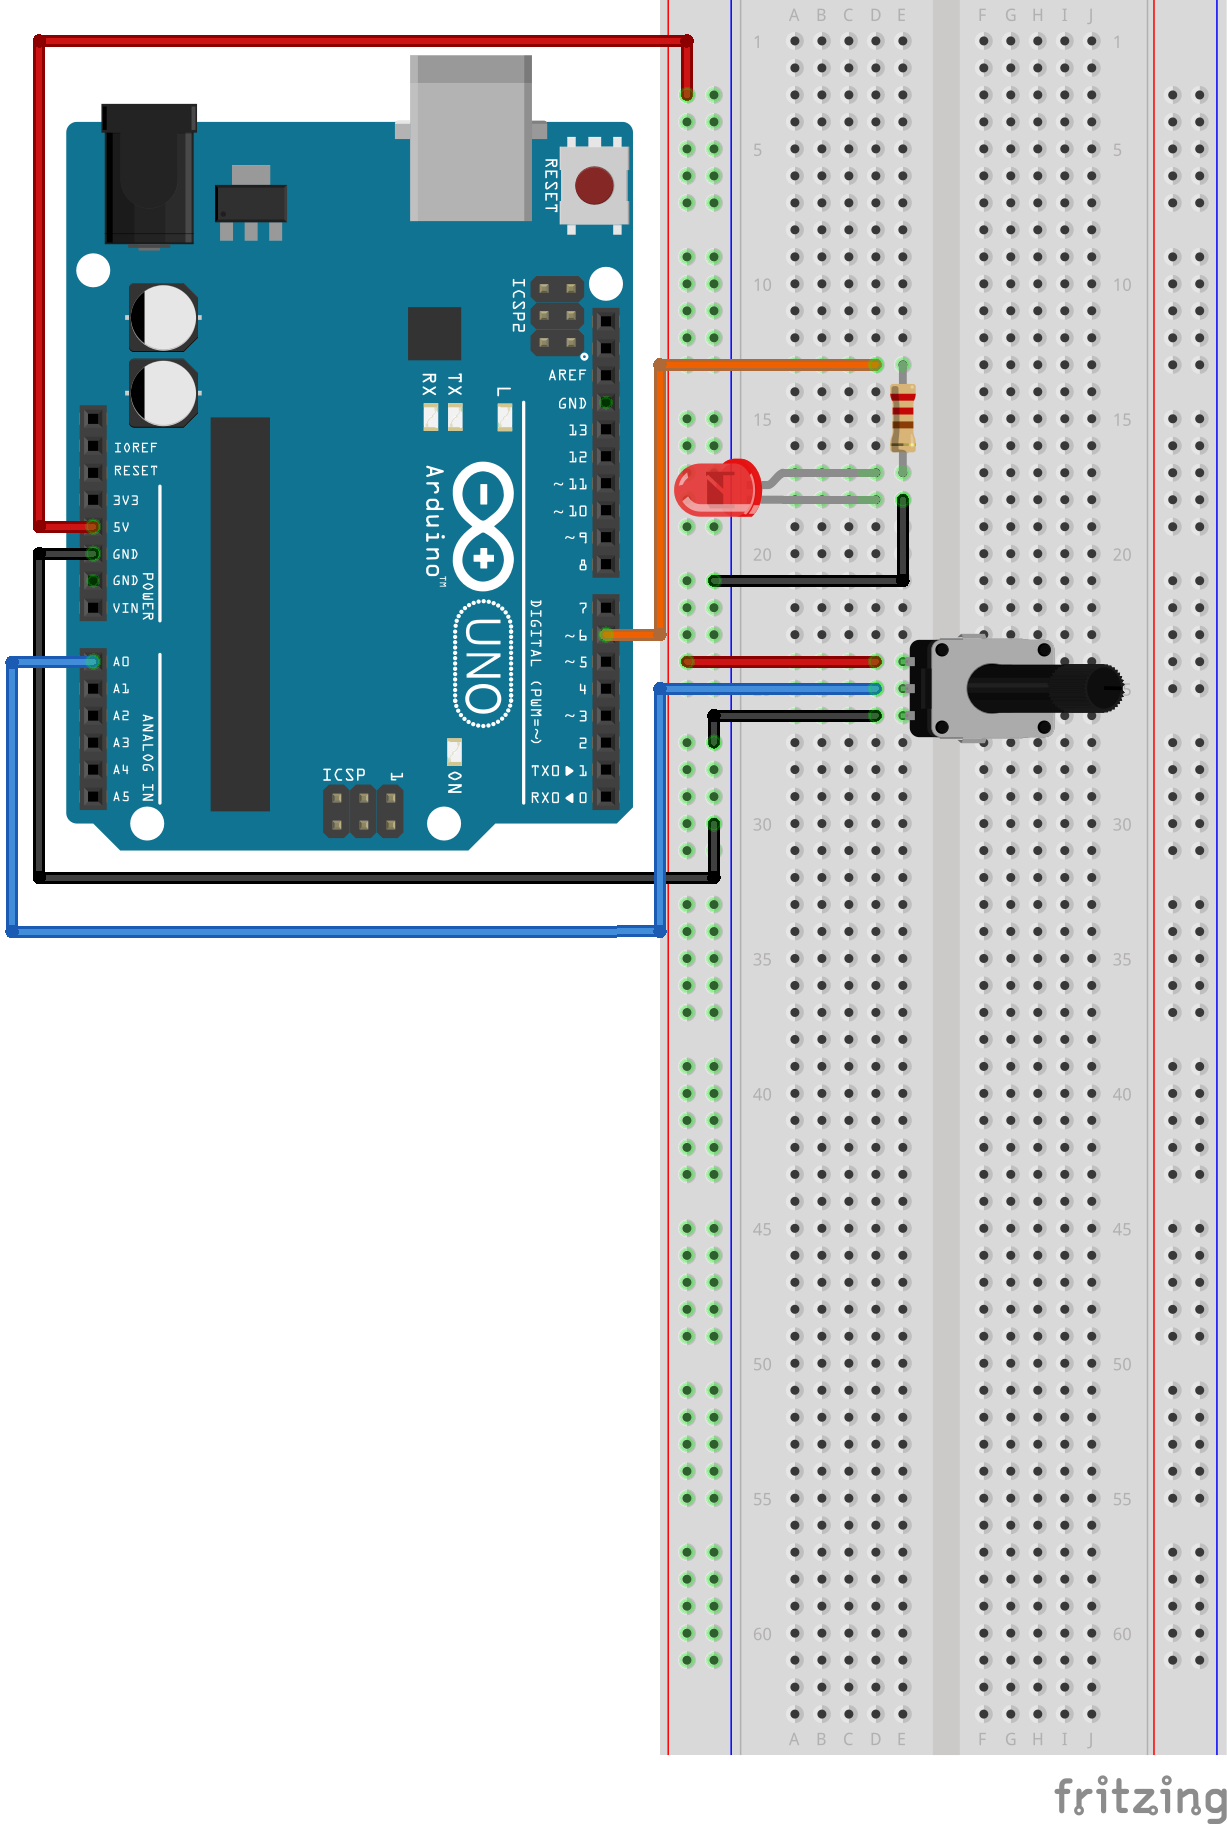
\includegraphics[width=1\textwidth]{../Examples/3_PotRead/3_PotRead_bb.png}
	\end{center}
	\end{column}
\end{columns}
\end{frame}
%%----------------------------------------------------------------------

\section{Kreative Opgaver}
%%----------------------------------------------------------------------
\begin{frame}{Kreative Opgaver}
	\begin{itemize}
	\item{Nu kan I starten af Arduino}
	\item{Opgaverne i dag kommer fra min Arduino Workshop}
	\item{Der ligger kreative opgaver tilgængelige, prøv at koble jeres udvidede C på:}
		\begin{itemize}
		\item{\color{link}\href{https://github.com/Iakop/C-Programmering-for-begyndere/tree/master/Del_4/Exercises/C_exercises_4_dansk.pdf}{../Del\_4/Exercises/C\_exercises\_4\_dansk.pdf}}
		\end{itemize}
	\item{Der er hjælp at hente her på workshoppen}
	\item{God arbejdslyst! - Happy Hacking!}
	\end{itemize}
\end{frame}
%%----------------------------------------------------------------------

\end{document}
